\setchapterimage[7.5cm]{images/marek-okon-N6JjTYisKRA-unsplash}
\setchapterpreamble[u]{\margintoc}
\chapter{Data Flow Testing}
\section{Basic Concepts}
The control flow testing strategy uses the program's control flow to identify the faults in a unit. The main emphasis of control flow testing is to execute the paths on the control flow to cover all statements, branches, and predicates. On the other hand, data flow testing deals with catching faults due to the changes in the variables through incorrect assignments, uninitialized variables, unused variables, and unintentionally making successive assignments of values to the same variable. 

Data flow testing can be performed at either static or dynamic levels, as with other unit testing methods. Static data flow testing is done by analyzing the code without running the program unit. Dynamic testing, on the other hand, is performed by running the program unit on the previously determined paths.

For representing these faults systematically, the following three terms are commonly used to identify the status of a variable during the execution of the code. 
\begin{enumerate}
    \item \textbf{Defined} (\textbf{d}): Variable is initialized using an assignment, an input statement, or by a parameter in a function call. For example, in $\textbf{a = b + 1}$, \textbf{a} is defined.
    \item \textbf{Referenced} or used (\textbf{r}): Variable is used on the right hand side of an assignment statement, or on the left hand side of an assignment as an index of an array, or in a predicate of a branching instruction. For example, in the if statement, $\textbf{if(list[m] == oldlist[n])}$, \textbf{list[m]}, \textbf{oldlist[n]}, and indices \textbf{m}, and \textbf{n} are referenced. Similarly, in $\textbf{a = b + 1}$, \textbf{b} is referenced (used).
    \item Killed or \textbf{Undefined} (\textbf{u}): Variable is used after its termination (e.g, by a \textbf{free()} statement in dynamic memory allocation in C), or undefined (uninitialized) before its first use). 
\end{enumerate}
The faults caused by the misuse of variables in the data flow are collectively named data anomalies\index{data anomalies} and are classified into three types using the sequences of actions defined by d, u, and r  as follows:
\begin{enumerate}
    \item \textbf{Type 1}. Defined and redefined (\textbf{dd\index{dd})}: This anomaly is caused as a result of (at least) two successive assignments without using the first  one. For example, in the following code segment, salary is defined and then redefined. One possibility is, unintentionally, instead of \textbf{totalSalary}, \textbf{salary} is used in the first occurrence. Another possibility is a missing statement or code segment between the two. Although this anomaly is generally considered harmless, it should be closely monitored and the cause of its occurrence should be explained.
    \begin{itemize}
        \item ...
        \item \textbf{salary} = computeGrossSalary(totalWeeklyEarnings);
        \item \textbf{salary} = computeNetSalary(totalSalary, taxDeduction); 
        \item ...
    \end{itemize}
    
    \item \textbf{Type 2}. Undefined but referenced (\textbf{ur\index{ur}}): This type of anomaly occurs as a result of uninitialized but later referenced variables. For example, assuming that variable \textbf{deduction} is not initialized (u), in the assignment statement, $\textbf{mygrade = mygrade - deduction;}$, the variable \textbf{deduction} is referenced (r), and hence causes \textbf{ur} type anomaly. This type of fault may have serious consequences and the initialization of a variable should not be left to the grace of a compiler.
    \item \textbf{Type 3}. Defined but not referenced (\textbf{du\index{du}}): This anomaly is caused by defining (declaring) a variable and undefining it without making any reference to it in the rest of the computation.  For example, if the value of \textbf{salary} defined by the assignment statement \textbf{salary=computeGrossSalary(totalWeeklyEarnings)} is never used in the rest of the code, this type of anomaly is observed. Coding resulting in this type of anomaly is considered a bad programming practice.
\end{enumerate}
Apparently, one can form 6 more binary combinations (\textbf{dr}, \textbf{ud}, \textbf{uu}, \textbf{rr}, \textbf{rr}, and \textbf{rd}) using the actions d, u, and r. These combinations do not cause any data flow anomaly.

\section{Data Flow Graph (DFG)}
In order to detect the anomalies, a path predicate expression should be derived for the path under consideration. For this purpose, the so called data flow graph\index{data flow graph} is utilized. A variable which is defined (d) in the code can be later used (r) on the right hand side of an assignment statement or in a predicate. These uses are names as c-use\index{c-use} (computation use), and \index{p-use} (predicate use) respectively.  

A data flow graph (DFG\index{DFG}) is a directed graph consisting of rectangular nodes and connecting edges with the following properties:
\begin{itemize}
    \item  Each node represents a sequence of data definitions and c-uses.
    \item A set of p-uses is associated with each edge.
    \item The entry node has a definition of each parameter and each non-local variable of the function (subprogram).
    \item The exit node (return from a function) has an undefinition (kill) of each local variable.
    \item A null node is used to represent the decision control point (if-then-else, for(), and while-do).
\end{itemize}

\begin{example}
For the C function \lstinline!isPalindrome! given in \refexample{state-branch-coverage}, draw a DFG.
\end{example}

\begin{marginfigure}
    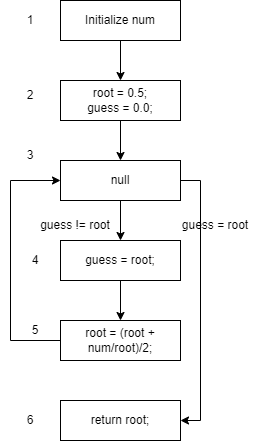
\includegraphics{images/dfg-2.png}
    \caption{Data flow graph for the Newton-Raphson iteration to compute the square root of a real number.}
    \labfig{dfg-2}
\end{marginfigure}

A DFG for \lstinline!isPalindrome! is given in \reffig{dfg-1}.
\begin{figure}[!ht]
    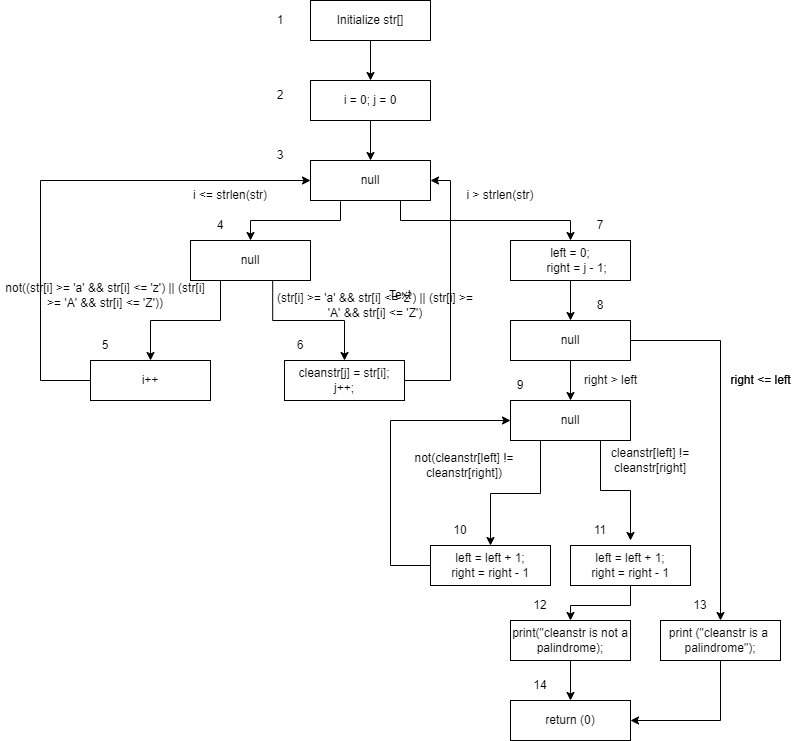
\includegraphics{images/dfg-1.png}
    \caption{Data flow graph for the program given in \refexample{state-branch-coverage}}.
    \labfig{dfg-1}
\end{figure}

\begin{example}
\labexample{squareRoot}
Square root of a non-negative number can be easily computed using the Newton-Raphson iteration formula. The C function below is an implementation of this technique to compute the square root of \textbf{num}. Create a a DFG, and identify the definitions, c-uses, and p-uses, of the variables \textbf{root}, \textbf{guess}, and \textbf{num}.

\begin{lstlisting}[language=C, caption={A C function to compute the positive square root of a real number.}]
double squareRoot(double num){
    double root = 1.0, guess = 0.0;
    while(guess != root){
        guess = root;
        root = (root + num/root) / 2.0;
    }
    return root;
}
\end{lstlisting}
\end{example}

A DFG is given in \reffig{dfg-2}. The definitions, c-uses, p-uses, and terminations (kill/undefine) of the three variables used in the function are shown in \reftab{def-use-term}.
\begin{table*}
    \begin{adjustbox}{max width=\linewidth}
        \begin{tabular}{ccccccccccccc}
            \toprule
            \thead{Line} & \multicolumn{4}{c}{\thead{root}} & \multicolumn{4}{c}{\thead{guess}} & \multicolumn{4}{c}{\thead{num}} \\
            \cmidrule(r){1-1}\cmidrule(lr){2-5}\cmidrule(lr){6-9}\cmidrule(l){10-13}
             & def & c-use & p-use & undef & def & c-use & p-use & undef & def & c-use & p-use & undef \\
            \cmidrule(lr){2-2}\cmidrule(lr){3-3}\cmidrule(lr){4-4}\cmidrule(lr){5-5}\cmidrule(lr){6-6}\cmidrule(lr){7-7}\cmidrule(lr){8-8}\cmidrule(lr){9-9}\cmidrule(lr){10-10}\cmidrule(lr){11-11}\cmidrule(lr){12-12}\cmidrule(l){13-13}
            1 &        &        &        &        &        & &        &        & \cmark &        & &        \\
            \midrule
            2 & \cmark &        &        &        & \cmark & &        &        &        &        & &        \\
            \midrule
            3 &        &        & \cmark &        &        & & \cmark &        &        &        & &        \\
            \midrule
            4 &        & \cmark &        &        & \cmark & &        &        &        &        & &        \\
            \midrule
            5 & \cmark & \cmark &        &        &        & &        &        &        & \cmark & &        \\
            \midrule
            6 &        &        &        &        &        & &        &        &        &        & &        \\
            \midrule
            7 &        & \cmark &        &        &        & &        &        &        &        & &        \\
            \midrule
            8 &        &        &        & \cmark &        & &        & \cmark &        &        & & \cmark \\
            \bottomrule
        \end{tabular}
    \end{adjustbox}
    \caption{Definitions, c-uses, p-uses and terminations (undefine) of the variables.}
    \labtab{def-use-term}
\end{table*}

Each variable in a function (unit) has a life-cycle which can be expressed as a sequence of events in terms of definition (def), c-use, p-use, and undefinition (undef) of it. For example, for the variable \textbf{root}, in the DFG given in  \reffig{dfg-2}, one can express the events as follows:
\begin{itemize}
    \item def(2)-(p-use(3)-c-use(4)-c-use(5), def(5))$^+$-undef(8), where '+' means one or more repetitions of the events in the bracket (node numbers on the DFG).
\end{itemize}
The goal of data flow testing is to generate test data in such a way as to execute all the paths that may have incorrect or suspicious event sequences (data anomalies). To explain the steps in data flow testing, two definitions will be used \autocite{mili2015software}:

\begin{definition}
\labdef{def-use}
A path in the program and on the corresponding DFG is a \textbf{definition-use path (du-path)}\index{definition-use path} for some variable x iff it starts with some statement that defines x and ends with a statement that uses (c-use or p-use) x.
\end{definition}

\begin{definition}
\labdef{def-clear}
A path in the program and on the corresponding DFG is a \textbf{definition-clear (def-clear) path}\index{definition-clear path} for some variable x iff it is a du-path for x and the definition statement (node) with which it starts is the only definition statement (node) for that variable in the path.
\end{definition}

For example, for the variable \textbf{root} in the example above, (2-3), (2-3(T)-4), (2-3(T)-4-5) are du-paths\index{du-paths}, and (2-3(T)-4) is a def-clear path\index{def-clear path}. 

Based on these definitions, one can describe the data flow testing process for a program (unit) as follows:
\begin{enumerate}
    \item Create a DFG corresponding to the program to be tested.
    \item Make a list of all the variables (input, function parameters, and others).
    \item For each variable of the program, list all the definitions, c-uses, and p-uses. 
    \item For each variable, determine a complete path (from the entry node to the exit node) including the def-use, and/or def-clear path for the variable. Determination of a path is based on different path selection criteria. In this book, only three of them will be mentioned as follows:
\begin{itemize}
    \item Use of \textbf{all du-paths}: According to this criteria, all du-paths are chosen including def-clear paths. 
    \item Use of \textbf{all c-uses}: According to this criteria, all c-use paths are chosen. A \textbf{c-use path}\index{c-use path} for a program with respect to a variable x, is a def-clear path from a definition of x to a c-use of x.  
    \item Use of \textbf{all p-uses}: According to this criteria, all pc-use paths are chosen. A \textbf{p-use path}\index{p-use path} for a program with respect to a variable x, is a def-clear path from a definition of x to a p-use of x. 
\end{itemize}
    \item For the selected path, first identify a complete path covering this path, and then obtain the corresponding path predicate, and the path predicate expression (see \refsec{gen-test-cases}).
    \item For dynamic data flow testing, to exercise this path, identify a complete path covering the c-use path, generate test data, and run the program.
\end{enumerate}

\begin{example}
Considering the function \lstinline!squareRoot! in \refexample{squareRoot}, and the variable \lstinline!root!, use \textbf{all c-uses} path selection criteria, to obtain a path predicate expression and a complete path covering the c-use path. Then, find a test input data to force the execution of this path.
\end{example}

By \refdef{def-clear},  (2-3(T)-4) is a def-clear and a c-use path with respect to the variable \lstinline!root!.The path predicate is \lstinline$guess != root$ $\equiv$ True. A complete (aggregate) path covering (2-3(T)-4) is (1-2-3(T)-4-5-3(F)-7). Interpretation of this path is given in \reftab{desc-int}.

\begin{table}
    \begin{adjustbox}{max width=\linewidth}
        \begin{tabular}{lll}
            \toprule
            \thead{Node} & \thead{Description} & \thead{Interpretation} \\
            \midrule
            1 & Input vector <num> & \\
            2 & \lstinline!root = 1.0, guess = 0.0! & \\
            3(T) & \lstinline$guess != root$ & \lstinline$0.0 != 1.0$ \\
            4 & \lstinline!guess = root! & \lstinline!guess = 1.0! \\
            5 & \lstinline!root = (root + num / root) / 2! & \lstinline!root = (1.0 + num / 1.0) / 2.0! \\
            6(F) & \lstinline$guess != root$ & \lstinline$1.0 != (1.0 + num / 1.0) / 2.0$ \\
            7 & \lstinline!return root! & \\
            \bottomrule
        \end{tabular}
    \end{adjustbox}
    \caption{This caption should be filled with an appropriate sentence.}
    \labtab{desc-int}
\end{table}

\todo{Tablo caption'ına placeholder koydum.}

A test input data to force the execution of this path is constructed as follows:
\begin{itemize}
    \item num = 1.0
    \item root = 1.0
    \item guess = 0.0
\end{itemize}
Observe that, for this input set, the body of the while loop is executed only once and the square root is obtained in one iteration of the Newton-Raphson method.

\section{Problems}
\begin{enumerate}
    \item Create a table of all possible binary combinations of d, u, and r actions for data flow anomalies. Give an example for each combination and state whether the combination causes an anomaly or not.
    \item  In C programming language, dynamic memory allocation and deallocation are possible using standard library functions \textbf{malloc()}, \textbf{calloc()}, \textbf{free()} and \textbf{realloc()}. Give an example for each of these library functions.
    \item Give an example of a Type1 data flow anomaly using the library functions given in the previous Exercise.
    \item Give an example of a Type2 data flow anomaly using the library functions given in the previous Exercise.
    \item Give an example of a Type3 data flow anomaly using the library functions given in the previous Exercise.
    \item For the DFG given in \reffig{dfg-1}, make a table consisting of all the variables and their uses (def, undef, c-use, and p-use).
     \item Using the table created in the previous question, use \textbf{all du-paths} criteria to  generate test data.
    \item Repeat the same for the \textbf{all c-uses} criteria to  generate test data.
    \item Repeat the same for the \textbf{all p-uses} criteria to  generate test data.
    \item Considering the function \lstinline!squareRoot! given in \refexample{squareRoot}, and the variable \lstinline!root!, use \textbf{all p-uses} path selection criteria, to obtain a path predicate expression and a complete path covering the p-use path. Then, find a test input data to force the execution of this path.
\end{enumerate}